\newcommand{\figureElectronicsLED}[1]{
  \def\lang{\detokenize{#1}}
  \def\langRu{\detokenize{ru}}
  \def\langEn{\detokenize{en}}
  \def\figureCaption{XXX: No translation.}
  \def\figureAnode{XXX: No translation.}
  \def\figureCathode{XXX: No translation.}
  \ifx \lang\langRu
  \def\figureCaption{
    Схематическое изображение одного из видов светодиода.
  }
  \def\figureAnode{Анод}
  \def\figureCathode{Катод}
  \fi
  \ifx \lang\langEn
  \def\figureCaption{
    An example of a vessel with a hole in the bottom.
  }
  \def\figureAnode{Anode}
  \def\figureCathode{Cathode}
  \fi
  \begin{figure}[ht]
    \centering
    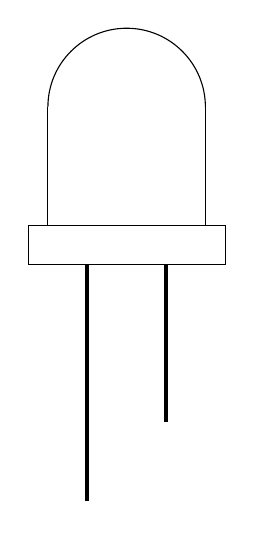
\begin{tikzpicture}
      \draw (0, 0) arc [
        start angle=0,
        end angle=180,
        x radius=1cm,
        y radius =1cm
      ];
      \draw (-2, 0) -- (-2, -1.5);
      \draw (0, 0) -- (0, -1.5);
      \draw (-2.25, -1.5) -- (0.25, -1.5) -- (0.25, -2.0) -- (-2.25, -2.0) -- (-2.25, -1.5);
      \draw[line width=0.5mm] (-1.5, -2.0) -- (-1.5, -5) node[left] {
        \figureAnode
      };
      \draw[line width=0.5mm] (-0.5, -2.0) -- (-0.5, -4) node[right] {
        \figureCathode
      };
    \end{tikzpicture}
    \caption{\figureCaption}
    \label{fig:electronics-led}
  \end{figure}
}
